% Fig. 3.2 -- joint pdf 的曲面，曲面之下所夾的體積即機率。
% 書稿來源: mathstatch3.tex 第 319 行的 tikzpicture。
%
% 幾何一律照書稿: view={50}{45}、domain 0:4、y domain 0:4、座標軸線不畫、
% 三軸都不標刻度，只留 x、y 與 z 三個軸名。
%
% 對書稿的三處調整:
%   1. colormap 由 whitegray 改為同色相的墨色濃淡 journalgray (CH3 規格 3.2)。
%   2. samples 由 50 改為 40 (CH3 規格 3.2 所定的產製規格)。
%   3. 字級: 書稿的 $f_{\sssig XY}$ 走 scriptscriptstyle，在 350px 顯示寬之下
%      下標只有 7.8px，未達 11px 門檻。此處改為一般下標，並以
%      \DeclareMathSizes 把 12pt 之下的 script 級撐到 10pt；圖寬同時由 11cm
%      收到 10.4cm。成圖的 viewBox 寬 249.96pt，在 350px 顯示寬之下
%      放大 1.400 倍，最小的字 (下標 XY，10pt) 為 13.9px。
%
% 產製 (CH3 規格 3.2 的三維曲面路徑，-O 不可省):
%   latex -interaction=nonstopmode '\def\pgfsysdriver{pgfsys-dvisvgm.def}% Fig. 3.2 -- joint pdf 的曲面，曲面之下所夾的體積即機率。
% 書稿來源: mathstatch3.tex 第 319 行的 tikzpicture。
%
% 幾何一律照書稿: view={50}{45}、domain 0:4、y domain 0:4、座標軸線不畫、
% 三軸都不標刻度，只留 x、y 與 z 三個軸名。
%
% 對書稿的三處調整:
%   1. colormap 由 whitegray 改為同色相的墨色濃淡 journalgray (CH3 規格 3.2)。
%   2. samples 由 50 改為 40 (CH3 規格 3.2 所定的產製規格)。
%   3. 字級: 書稿的 $f_{\sssig XY}$ 走 scriptscriptstyle，在 350px 顯示寬之下
%      下標只有 7.8px，未達 11px 門檻。此處改為一般下標，並以
%      \DeclareMathSizes 把 12pt 之下的 script 級撐到 10pt；圖寬同時由 11cm
%      收到 10.4cm。成圖的 viewBox 寬 249.96pt，在 350px 顯示寬之下
%      放大 1.400 倍，最小的字 (下標 XY，10pt) 為 13.9px。
%
% 產製 (CH3 規格 3.2 的三維曲面路徑，-O 不可省):
%   latex -interaction=nonstopmode '\def\pgfsysdriver{pgfsys-dvisvgm.def}% Fig. 3.2 -- joint pdf 的曲面，曲面之下所夾的體積即機率。
% 書稿來源: mathstatch3.tex 第 319 行的 tikzpicture。
%
% 幾何一律照書稿: view={50}{45}、domain 0:4、y domain 0:4、座標軸線不畫、
% 三軸都不標刻度，只留 x、y 與 z 三個軸名。
%
% 對書稿的三處調整:
%   1. colormap 由 whitegray 改為同色相的墨色濃淡 journalgray (CH3 規格 3.2)。
%   2. samples 由 50 改為 40 (CH3 規格 3.2 所定的產製規格)。
%   3. 字級: 書稿的 $f_{\sssig XY}$ 走 scriptscriptstyle，在 350px 顯示寬之下
%      下標只有 7.8px，未達 11px 門檻。此處改為一般下標，並以
%      \DeclareMathSizes 把 12pt 之下的 script 級撐到 10pt；圖寬同時由 11cm
%      收到 10.4cm。成圖的 viewBox 寬 249.96pt，在 350px 顯示寬之下
%      放大 1.400 倍，最小的字 (下標 XY，10pt) 為 13.9px。
%
% 產製 (CH3 規格 3.2 的三維曲面路徑，-O 不可省):
%   latex -interaction=nonstopmode '\def\pgfsysdriver{pgfsys-dvisvgm.def}% Fig. 3.2 -- joint pdf 的曲面，曲面之下所夾的體積即機率。
% 書稿來源: mathstatch3.tex 第 319 行的 tikzpicture。
%
% 幾何一律照書稿: view={50}{45}、domain 0:4、y domain 0:4、座標軸線不畫、
% 三軸都不標刻度，只留 x、y 與 z 三個軸名。
%
% 對書稿的三處調整:
%   1. colormap 由 whitegray 改為同色相的墨色濃淡 journalgray (CH3 規格 3.2)。
%   2. samples 由 50 改為 40 (CH3 規格 3.2 所定的產製規格)。
%   3. 字級: 書稿的 $f_{\sssig XY}$ 走 scriptscriptstyle，在 350px 顯示寬之下
%      下標只有 7.8px，未達 11px 門檻。此處改為一般下標，並以
%      \DeclareMathSizes 把 12pt 之下的 script 級撐到 10pt；圖寬同時由 11cm
%      收到 10.4cm。成圖的 viewBox 寬 249.96pt，在 350px 顯示寬之下
%      放大 1.400 倍，最小的字 (下標 XY，10pt) 為 13.9px。
%
% 產製 (CH3 規格 3.2 的三維曲面路徑，-O 不可省):
%   latex -interaction=nonstopmode '\def\pgfsysdriver{pgfsys-dvisvgm.def}\input{joint-pdf-surface.tex}'
%   dvisvgm -O -d2 -n -o ../../images/teaching-topics/joint-pdf-surface.svg joint-pdf-surface.dvi

\documentclass[tikz,border=2pt]{standalone}
\usepackage{amsmath}
\usepackage{amssymb}
\usepackage{xcolor}
\usepackage{pgfplots}
\pgfplotsset{compat=1.18}

\definecolor{journalink}{HTML}{1F1C18}
\definecolor{journalmuted}{HTML}{8A7F72}
\definecolor{journalaccent}{HTML}{9C2D2D}

%% 12pt (即 \large) 之下的 script 級撐到 10pt，
%% 使 f 的下標 XY 在 350px 顯示寬之下仍在 11px 之上。
\DeclareMathSizes{12}{12}{10}{8}

%% 書稿用 whitegray 灰階曲面; 本站改用同一色相的墨色濃淡，
%% 與其他圖的主線色 journalink 相稱。
\pgfplotsset{
  colormap={journalgray}{color(0cm)=(white); color(1cm)=(journalink)}
}

\begin{document}
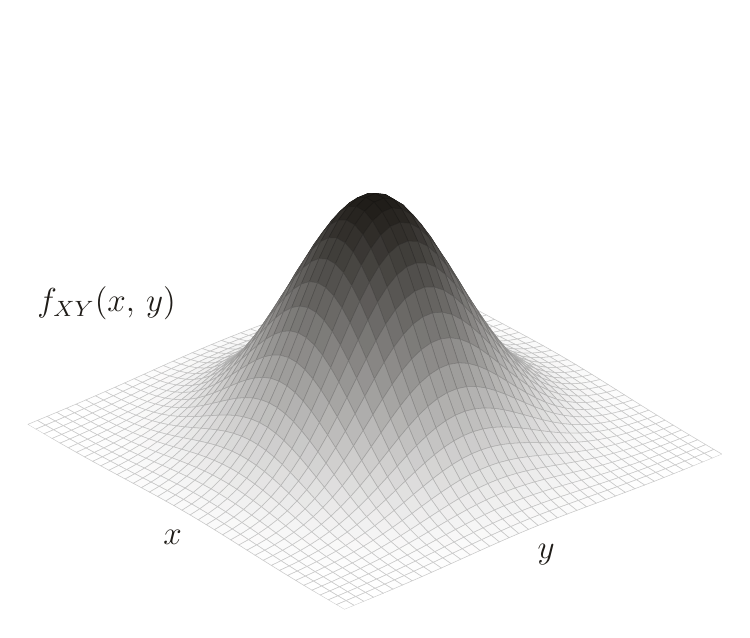
\begin{tikzpicture}[
    declare function={mu1=2;},
    declare function={mu2=2;},
    declare function={sigma1=1;},
    declare function={sigma2=1;},
    declare function={bivar(\ma,\sa,\mb,\sb)=
        1/(2*pi*\sa*\sb) * exp(-((x-\ma)^2/\sa^2 + (y-\mb)^2/\sb^2))/2;}]
\begin{axis}[
    axis line style={draw=none},
    colormap name=journalgray,
    width=10.4cm,
    view={50}{45},
    enlargelimits=false,
    domain=0:4,
    y domain=0:4,
    samples=40,
    xlabel=$x$,
    ylabel=$y$,
    zlabel={$f_{XY}(x,\,y)$},
    label style={journalink, font=\large},
    xtick=\empty,
    ytick=\empty,
    ztick=\empty,
    zlabel style={rotate=-90, anchor=west},
]
\addplot3[surf, draw=journalink, line width=0.2pt] {bivar(mu1,sigma1,mu2,sigma2)};
\end{axis}
\end{tikzpicture}
\end{document}
'
%   dvisvgm -O -d2 -n -o ../../images/teaching-topics/joint-pdf-surface.svg joint-pdf-surface.dvi

\documentclass[tikz,border=2pt]{standalone}
\usepackage{amsmath}
\usepackage{amssymb}
\usepackage{xcolor}
\usepackage{pgfplots}
\pgfplotsset{compat=1.18}

\definecolor{journalink}{HTML}{1F1C18}
\definecolor{journalmuted}{HTML}{8A7F72}
\definecolor{journalaccent}{HTML}{9C2D2D}

%% 12pt (即 \large) 之下的 script 級撐到 10pt，
%% 使 f 的下標 XY 在 350px 顯示寬之下仍在 11px 之上。
\DeclareMathSizes{12}{12}{10}{8}

%% 書稿用 whitegray 灰階曲面; 本站改用同一色相的墨色濃淡，
%% 與其他圖的主線色 journalink 相稱。
\pgfplotsset{
  colormap={journalgray}{color(0cm)=(white); color(1cm)=(journalink)}
}

\begin{document}
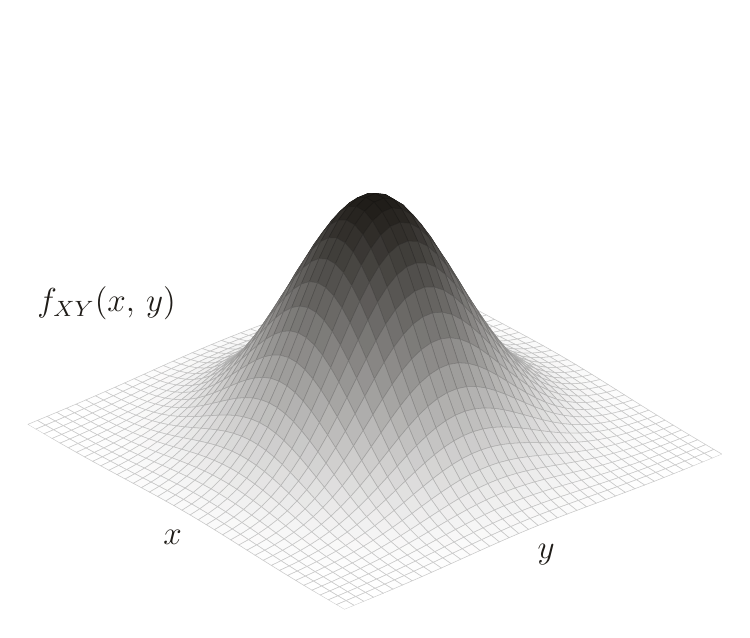
\begin{tikzpicture}[
    declare function={mu1=2;},
    declare function={mu2=2;},
    declare function={sigma1=1;},
    declare function={sigma2=1;},
    declare function={bivar(\ma,\sa,\mb,\sb)=
        1/(2*pi*\sa*\sb) * exp(-((x-\ma)^2/\sa^2 + (y-\mb)^2/\sb^2))/2;}]
\begin{axis}[
    axis line style={draw=none},
    colormap name=journalgray,
    width=10.4cm,
    view={50}{45},
    enlargelimits=false,
    domain=0:4,
    y domain=0:4,
    samples=40,
    xlabel=$x$,
    ylabel=$y$,
    zlabel={$f_{XY}(x,\,y)$},
    label style={journalink, font=\large},
    xtick=\empty,
    ytick=\empty,
    ztick=\empty,
    zlabel style={rotate=-90, anchor=west},
]
\addplot3[surf, draw=journalink, line width=0.2pt] {bivar(mu1,sigma1,mu2,sigma2)};
\end{axis}
\end{tikzpicture}
\end{document}
'
%   dvisvgm -O -d2 -n -o ../../images/teaching-topics/joint-pdf-surface.svg joint-pdf-surface.dvi

\documentclass[tikz,border=2pt]{standalone}
\usepackage{amsmath}
\usepackage{amssymb}
\usepackage{xcolor}
\usepackage{pgfplots}
\pgfplotsset{compat=1.18}

\definecolor{journalink}{HTML}{1F1C18}
\definecolor{journalmuted}{HTML}{8A7F72}
\definecolor{journalaccent}{HTML}{9C2D2D}

%% 12pt (即 \large) 之下的 script 級撐到 10pt，
%% 使 f 的下標 XY 在 350px 顯示寬之下仍在 11px 之上。
\DeclareMathSizes{12}{12}{10}{8}

%% 書稿用 whitegray 灰階曲面; 本站改用同一色相的墨色濃淡，
%% 與其他圖的主線色 journalink 相稱。
\pgfplotsset{
  colormap={journalgray}{color(0cm)=(white); color(1cm)=(journalink)}
}

\begin{document}
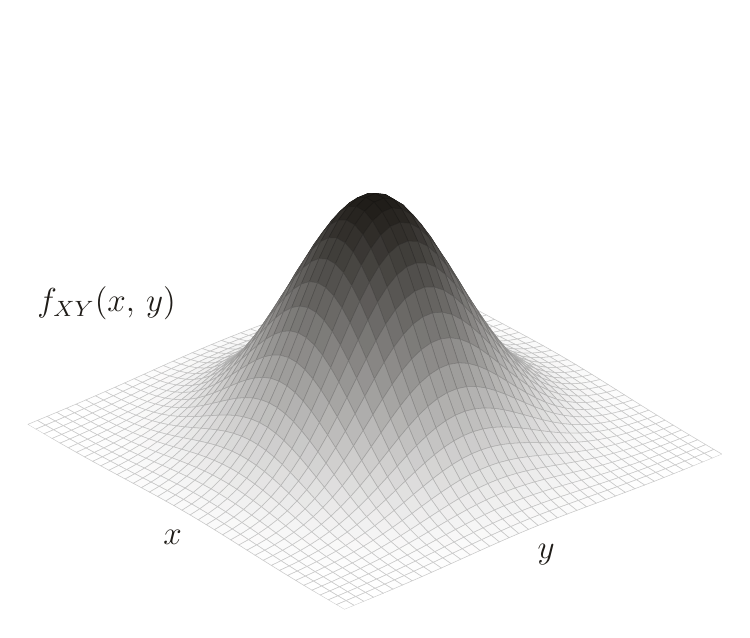
\begin{tikzpicture}[
    declare function={mu1=2;},
    declare function={mu2=2;},
    declare function={sigma1=1;},
    declare function={sigma2=1;},
    declare function={bivar(\ma,\sa,\mb,\sb)=
        1/(2*pi*\sa*\sb) * exp(-((x-\ma)^2/\sa^2 + (y-\mb)^2/\sb^2))/2;}]
\begin{axis}[
    axis line style={draw=none},
    colormap name=journalgray,
    width=10.4cm,
    view={50}{45},
    enlargelimits=false,
    domain=0:4,
    y domain=0:4,
    samples=40,
    xlabel=$x$,
    ylabel=$y$,
    zlabel={$f_{XY}(x,\,y)$},
    label style={journalink, font=\large},
    xtick=\empty,
    ytick=\empty,
    ztick=\empty,
    zlabel style={rotate=-90, anchor=west},
]
\addplot3[surf, draw=journalink, line width=0.2pt] {bivar(mu1,sigma1,mu2,sigma2)};
\end{axis}
\end{tikzpicture}
\end{document}
'
%   dvisvgm -O -d2 -n -o ../../images/teaching-topics/joint-pdf-surface.svg joint-pdf-surface.dvi

\documentclass[tikz,border=2pt]{standalone}
\usepackage{amsmath}
\usepackage{amssymb}
\usepackage{xcolor}
\usepackage{pgfplots}
\pgfplotsset{compat=1.18}

\definecolor{journalink}{HTML}{1F1C18}
\definecolor{journalmuted}{HTML}{8A7F72}
\definecolor{journalaccent}{HTML}{9C2D2D}

%% 12pt (即 \large) 之下的 script 級撐到 10pt，
%% 使 f 的下標 XY 在 350px 顯示寬之下仍在 11px 之上。
\DeclareMathSizes{12}{12}{10}{8}

%% 書稿用 whitegray 灰階曲面; 本站改用同一色相的墨色濃淡，
%% 與其他圖的主線色 journalink 相稱。
\pgfplotsset{
  colormap={journalgray}{color(0cm)=(white); color(1cm)=(journalink)}
}

\begin{document}
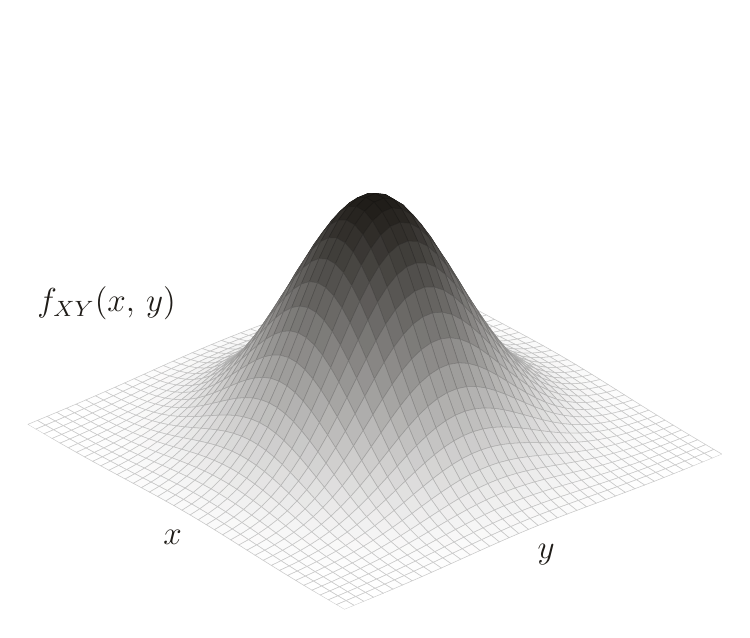
\begin{tikzpicture}[
    declare function={mu1=2;},
    declare function={mu2=2;},
    declare function={sigma1=1;},
    declare function={sigma2=1;},
    declare function={bivar(\ma,\sa,\mb,\sb)=
        1/(2*pi*\sa*\sb) * exp(-((x-\ma)^2/\sa^2 + (y-\mb)^2/\sb^2))/2;}]
\begin{axis}[
    axis line style={draw=none},
    colormap name=journalgray,
    width=10.4cm,
    view={50}{45},
    enlargelimits=false,
    domain=0:4,
    y domain=0:4,
    samples=40,
    xlabel=$x$,
    ylabel=$y$,
    zlabel={$f_{XY}(x,\,y)$},
    label style={journalink, font=\large},
    xtick=\empty,
    ytick=\empty,
    ztick=\empty,
    zlabel style={rotate=-90, anchor=west},
]
\addplot3[surf, draw=journalink, line width=0.2pt] {bivar(mu1,sigma1,mu2,sigma2)};
\end{axis}
\end{tikzpicture}
\end{document}
